A helpdesk alkalmazás \aref{ch:uzleti_igenyek}. fejezetben leírtaknak megfelelően szolgál ki három különböző e-mail címet:

\begin{itemize}
	\item a \textit{generic} sorhoz tarozó  \href{mailto:helpdesk.gdf@yandex.com}{\nolinkurl{helpdesk.gdf@yandex.com}}-ot, 
	\item a \textit{travel} sorhoz tarozó  \href{mailto:helpdesk.gdf.travel@yandex.com}{\nolinkurl{helpdesk.gdf.travel@yandex.com}}-ot,
	\item és a \textit{theater} sorhoz tarozó  \href{mailto:h.gdf.theater@gmx.com}{\nolinkurl{h.gdf.theater@gmx.com}}-ot.
\end{itemize}



\section{Alkalmazás elindítása}\label{sec:elinditas}
Az alakalmazás a \textit{start.sh} bash \textit{script}tel indítható el. A \textit{script} két dolgot csinál:
\begin{enumerate}
	\item a \textit{docker-compose} parancssal elindítja a docker \textit{container}eket~(\ref{sec:docker} pont),
	\item  ``helpdesk'' domain névvel hozzáadja a loadbalancer (\ref{sec:nginx} pont) IP címét a \mbox{\textit{/etc/hosts}} állományhoz.
\end{enumerate}

A \textit{script} indítása után a helpdesk alkalmazás elérhető a  \href{http://helpdesk}{http://helpdesk} domain alatt.


\section{Több példány}
A különböző szervizekből a terhelésnek megfelelően eltérő számú példány indul el:

\begin{itemize}
	\item a helpdesk-backendből három,
	\item a \textit{theater} sort kezelő email-kliensből egy,
	\item a \textit{travel} sort kezelő email-kliensből kettő,
	\item a \textit{generic} sort kezelő email-kliensből három,
	\item és a Kafka brókerből szintén három darab.
\end{itemize}

A példányok metrikáit (\ref{sec:metrikak} pont) nyomon lehet követni az erre a célra létrehozott Grafana oldalon (todo ábra). Az oldal elérhető a  \textit{Spring metrics} menüpont alatt.

Az todo ábrán csak a Grafana oldal legfelső néhány panele látható, az instance-okra lebontott legfontosabb mérőszámok:

\begin{itemize}
	\item a legfelső sorban a Java Virtual Machine, által akutálisan felhasznált Heap space,	
	\item alatta az aktuális REST lekérések száma,
	\item a harmadik sorban a feldolgozott Kafka üzenetk száma,
	\item míg az utolsó sorban a Trace logüzenetek száma látható.
\end{itemize}


\section{Deployment}
A könyebb bemutathatóság érdekében a szemléletesebb szervizeket --hogy ne a docker daemon által kiosztott IP címen keresztül kelljen elérni-- a docker hálózaton kívül is elérhetővé tettem. 

A \textit{docker-compose} (\ref{sec:elinditas}) által elindított \textit{container}eket \aref{fig:deployment_diagram}. ábrán foglaltam össze. Az ábrán feltüntettem, hogy az adott \textit{container}t a \textit{localhost} melyik portján lehet elérni.


\begin{figure}[hbt] 
	\centering
	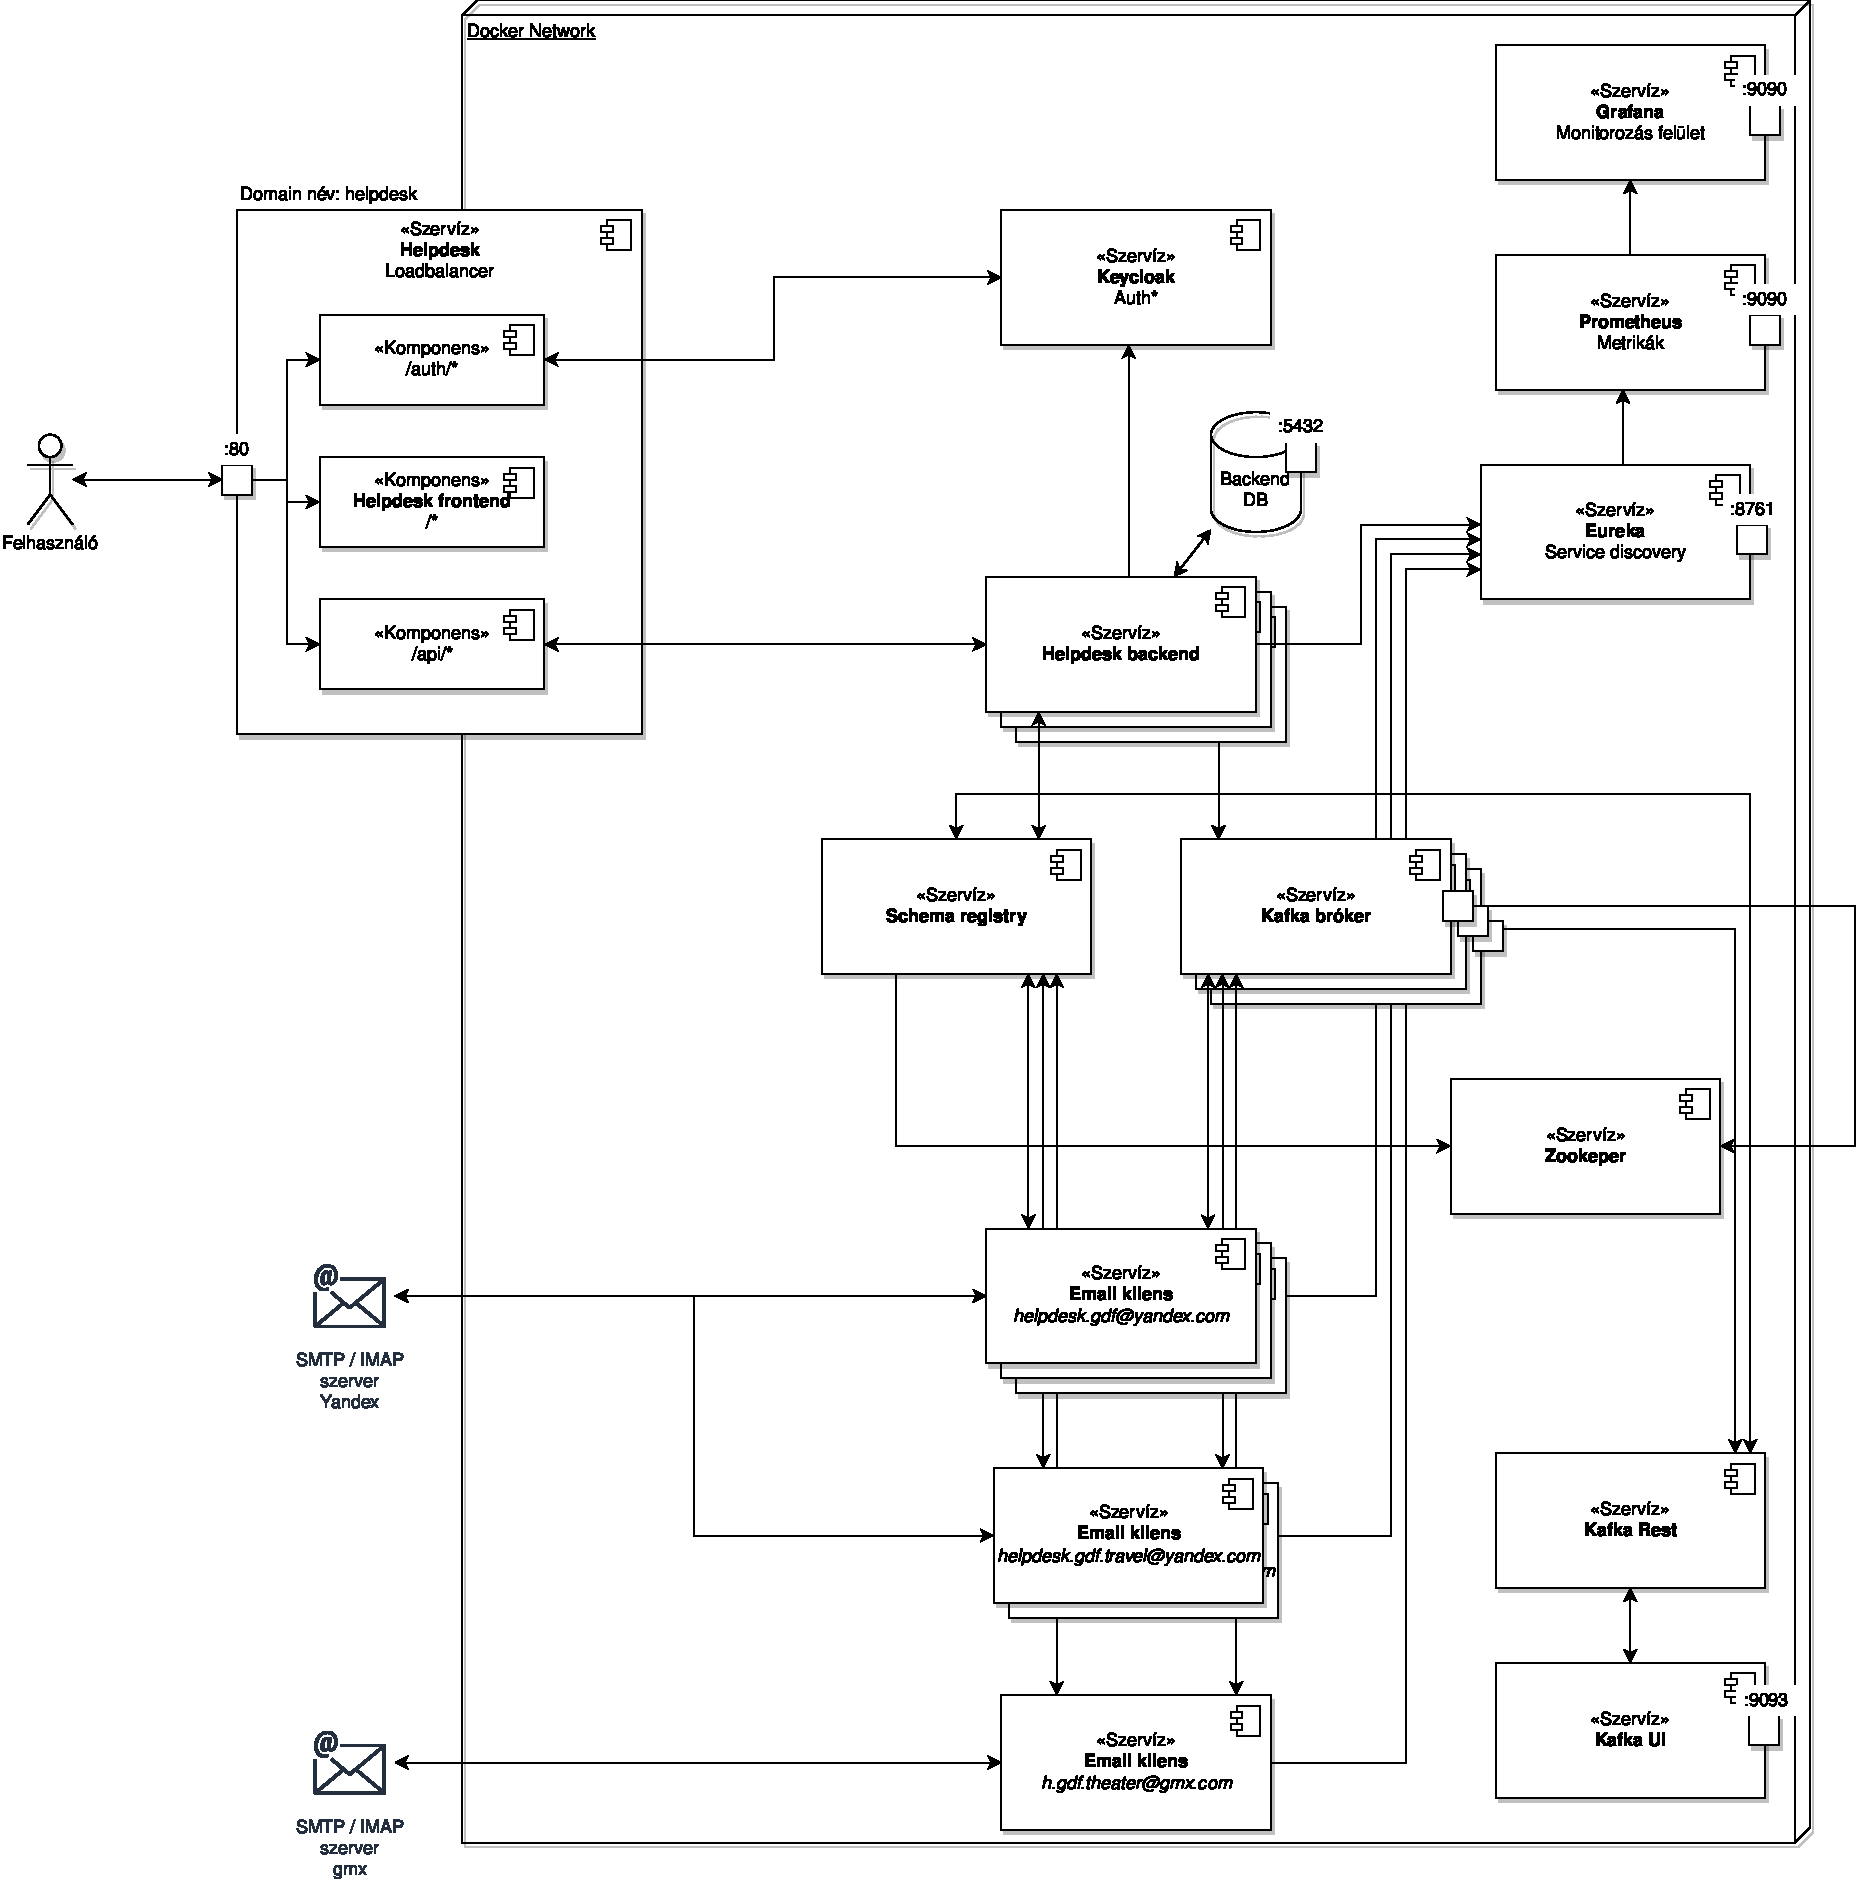
\includegraphics[width=0.85\textwidth]{deployment_diagram_drawio.pdf}
	\caption[Deployment diagram]{Deployment diagram}
	\label{fig:deployment_diagram}
	\floatfoot{Forrás: saját ábra}
\end{figure}


\section{Load test}
Jmeter load test

\section{Egy e-mail útja}
message flow diagram

\section{Felhasználói felület funkciói}
 képenyőképek? valami how to dokumentáció	

\section{Kafka topicok?}
a replication factorról meg a három brókerről
topicok meg egyebek